%!TEX root = P231_notes.tex

\section{Complex Analysis Review}
\lecdate{lec~12}

\subsection{Teaser: why are we doing this?}

We now switch gears to complex analysis. One of the results that I hope you'll come to appreciate in your study of physics is the rich role of complex numbers (and their generalizations) in describing nature. Our study of complex analysis will focus on motivating the residue theorem to calculate integrals in complex space. This, in turn, is useful when we represent functions in \emph{momentum space} by Fourier transforming. For example, a Green's function $G(x,x')$ can be written with respect to the Fourier momentum variable $k$ by
\begin{align}
	G(x,x') &= \int \dbar k \, e^{-ikx} \tilde G(k,x') \ ,
	\label{eq:complex:intro:G:fourier}
\end{align}
where I've used a convenient notation where $\dbar = d/2\pi$. This, in turn is useful because our defining relation for the Green's function is \eqref{eq:Greens:func:as:inverse}:
\begin{align}
	\mathcal O_xG(x,x') &= \delta(x-x') \ ,
\end{align}
which we may then write (Fourier transforming both sides) as
\begin{align}
	\mathcal O_x \int \dbar k \, e^{-ikx} \tilde G(k,x') 
	=
	\int \dbar k \, e^{-ikx} e^{ikx'} \ .
	\label{eq:complex:intro:defining:G:}
\end{align}
On the right-hand side we've written the $\delta(x-x')$ in its Fourier representation. We have assumed that $\mathcal O_x$ is a polynomial in derivatives with respect to $x$:
\begin{align}
	\mathcal O_x = \sum_{n=0}^{\infty}
	p_n(x) \left(\frac{d}{dx}\right)^n
	\equiv P\left(x,\frac{d}{dx}\right) \ .
	\label{eq:complex:intro:defining:Ox}
\end{align}
What's powerful about this is that that when we apply a differential operator in $x$ onto the Fourier representation of a function, say \eqref{eq:complex:intro:G:fourier}, then the derivatives only `see' the exponential factor $e^{-ikx}$. This means that derivatives are particularly easy:
\begin{align}
	\left(\frac{d}{dx}\right)^n e^{-ikx} &= (-ik)^n \ .
\end{align}
This means that we may write the differential operator $\mathcal O_x$ in \eqref{eq:complex:intro:defining:Ox} when it acts on the Fourier representation as
\begin{align}
	\mathcal O_x = \sum_{n=0}^{\infty}
	p_n(x) \left(-ik\right)^n
	\equiv P\left(x,-ik\right)  \ ,
\end{align}
so that the defining relation for $G$,
\eqref{eq:complex:intro:defining:G:}, may in turn be simplified:
\begin{align}
	\int \dbar k \, e^{-ikx} P(x, -ik) \tilde G(k,x') &= \int \dbar k \, e^{-ik(x-x')} \ ,
\end{align}
which suggests a simple expression for the Fourier coefficients:
\begin{align}
	\tilde G(k,x') &= e^{ikx'} \left[P(x,-ik)\right]^{-1} \ ,
\end{align}
where one may find $G(x,x')$ from simply taking the inverse Fourier transform. There will turn out to be a few neat features of this approach, but before getting there, let's start from the very beginning.

\lecdate{lec~13} % or Lec 11 of 2017

\subsection{Complex Numbers}

A complex number $z$ may be decomposed into real and imaginary parts
\begin{align}
	z = x + i y \ ,
\end{align}
where $x$ and $y$ are both real numbers. We may also define the complex conjugate as
\begin{align}
	\bar z = z^* = x - i y \ .
\end{align}
One may also write these variables in a polar notation,
\begin{align}
	z &= re^{i\theta}
	&
	\bar z &= re^{-i\theta} \ ,
\end{align}
where $r \in [0,\infty]$ and $\theta \in [0, 2\pi]$:
\begin{center}
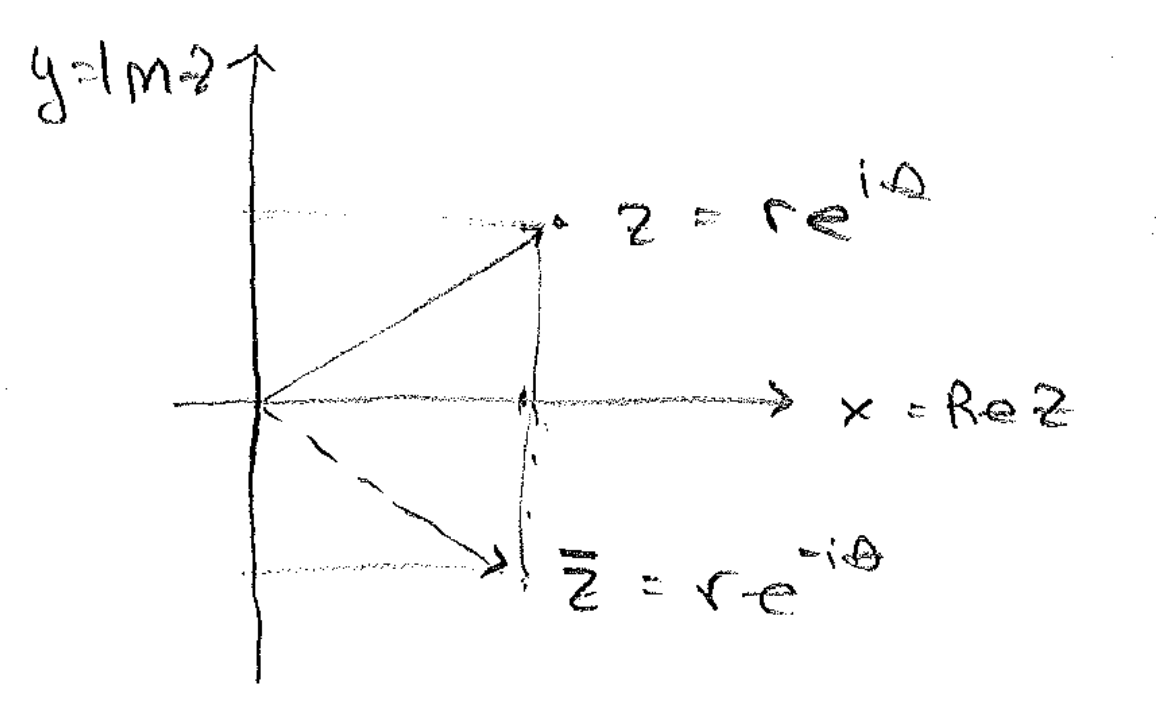
\includegraphics[width=.5\textwidth]{lec13_complexvar}
\end{center}
Complex numbers live in the space of complex numbers $\mathbbm{C}$, a \emph{two-dimensional} real space with coordinates $(x,y)$ in $\mathbbm{R}^2$ augmented by an additional rule for multiplication (take two complex numbers and return a complex number) that is called the \emph{complex structure}. This is basically the definition $i^2 = -1$, though one may generalize to higher complex dimensions. 


\subsection{Complex functions}

Complex functions take complex numbers and return complex numbers. Inspired by the two-dimensional-ness of $\mathbbm{C}$, let us write a complex function as $f(z)=f(x,y)$ where $z = x+i y$. Because $f(x,y)$ is, itself, a complex number for a given $z=x+i y$, we can decompose $f$ into two real-valued functions
\begin{align}
	f(z) = f(x,y) &= u(x,y) + i v(x,y) \ .
\end{align}
This is clearly a map from $\mathbbm{C} \to \mathbbm{C}$ and so we can simply ``do multivariable calculus'' on this space. 

If we forget the complex structure, then this \emph{seems} to simply be the calculus of maps between $\mathbbm{R}^2 \to \mathbbm{R}^2$ where
\begin{align}
	f(x,y) &= u(x,y) \hat{\vec{x}} + v(x,y)\hat{\vec{y}} \ .
\end{align}
In that case, we need to collect the partial derivatives. We know that we can write the variation of $f$ as
\begin{align}
\delta f(x,y) &= \delta u(x,y) \hat{\vec{x}} + \delta v(x,y)\hat{\vec{y}} 
=
\left(
	\frac{\partial u}{\partial x}\delta x +
	\frac{\partial u}{\partial y}\delta y
\right)\hat{\vec{x}}+
\left(
	\frac{\partial v}{\partial x}\delta x +
	\frac{\partial v}{\partial y}\delta y
\right)\hat{\vec{y}} \ .
\end{align}
Remembering our complex structure, we can write this succinctly as
\begin{align}
	\delta f &= 
	\frac{\partial f}{\partial z}\delta z +
	\frac{\partial f}{\partial \bar z}\delta \bar z \ ,
	\label{eq:complex:2D:deviation}
\end{align}
where we're using
\begin{align}
	\frac{\partial}{\partial z} &= 
	\frac{1}{2}
	\left(
	\frac{\partial}{\partial x}
	+
	\frac{\partial}{\partial (iy)}
	\right)
	&
	\frac{\partial}{\partial \bar z} &= 
	\frac{1}{2}
	\left(
	\frac{\partial}{\partial x}
	+
	\frac{\partial}{\partial (-iy)}
	\right) 
	\\
	&=
	\frac{1}{2}
	\left(
	\frac{\partial}{\partial x}
	-i
	\frac{\partial}{\partial y}
	\right)
	&
	\frac{\partial}{\partial \bar z} &= 
	\frac{1}{2}
	\left(
	\frac{\partial}{\partial x}
	+i
	\frac{\partial}{\partial y}
	\right) 
	\ .
\end{align}
The fact that partial derivatives combine like this may be familiar\footnote{This comes from the underlying mathematical structure. The partial derivatives are basis vectors for the \emph{tangent space} at some point $(x,y)$. These partial derivatives ask: how much does the function I'm acting on change if I move by one unit in this direction?}. 

So far we have emphasized that $f(x,y)$ behaves like a function in two real dimensions. Critically, in some ways we want to think about functions $f(z)$ that are functions of `one' [complex] dimension rather than two real dimensions. In two real dimensions, calculus came with a notion of directional derivative. When we wanted the rate of change for a function, we had to ask \emph{in what direction} are we checking the rate of change. At a given function may change by a positive amount in the $x$-direction, but a negative amount in the $y$-direction, for example. This is in contrast to one-dimensional calculus where each point had an unambiguous derivative that represented how much the function changed in the positive $x$ direction with respect to a point $x_0$:
\begin{align}
	\delta f(x) = \frac{d f(x_0)}{d x} (x-x_0) + \cdots \ .
\end{align}
This is in contrast to the change in a general complex function \eqref{eq:complex:2D:deviation}. In fact, if we explicitly wrote some expansion with respect to a point $z_0$, it looks a little funny:
\begin{align}
	\delta f(z) &= 
	\frac{\partial f}{\partial z}(z-z_0) +
	\frac{\partial f}{\partial \bar z}(\bar z-\bar z_0) + \cdots \ .
\end{align}
What is going on here? Why should $f(z)$ be a function of one complex variable $z$ but the expansion seems to depend not only on $(z-z_0)$ but also $(z-z_0)^*$?

\subsection{Analytic complex functions are nice}

This leads us to a definition of ``nice'' complex functions. The following terms are all more-or-less equivalent for this sense of nice-ness: \textbf{[complex] differentiable}, \textbf{analytic}, \textbf{holomorphic}, \textbf{regular}. This is simply the restriction that the $\partial f/\partial \bar z$ term should vanish so that the variation $f(z)$ only depends on $\delta z$ and not $\delta\bar z$. In other words, an analytic function admits usual single-dimensional definition of the derivative,
\begin{align}
	\frac{df(z_0)}{dz} &= \lim_{z\to z_0} \frac{f(z)-f(z_0)}{z-z_0} \ .
	\label{eq:df:dz:analytic:def}
\end{align}
The key aspect of this is that there is only \emph{one} value of $df/dz$ at $z_0$ no matter how you approach $z_0$. In other words, it doesn't matter if $\delta z = z-z_0$ is coming from the positive/negative real/imaginary direction. The value of $df/dz$ is the same. 

For most of these lectures we will use the term \textbf{analytic} to refer this property. Let us see what happens when we impose $df/d\bar{z} = 0$ onto the component functions $u(x,y)$ and $v(x,y)$:
\begin{align}
	\frac{1}{2}\left(\frac{\partial}{\partial x} + i \frac{\partial}{\partial y}\right)
	\left[u(x,y)+iv(v,y)\right]
	&= 
	\frac{1}{2}
	\left( \frac{\partial u}{\partial x} - \frac{\partial v}{\partial y} \right)
	+
	\frac{i}{2}
	\left( \frac{\partial u}{\partial y} + \frac{\partial v}{\partial x} \right)
	= 0 \ .
\end{align}
This implies the \textbf{Cauchy--Riemann equations}, which are equivalent to the function $f$ being analytic:
\begin{align}
	\frac{\partial u}{\partial x} & = +\frac{\partial v}{\partial y}
	&
	\frac{\partial u}{\partial y} & = -\frac{\partial v}{\partial x} \ .
\end{align}

Thus far we've talked about functions being analytic or not. It turns out that analytic functions are \emph{so} nice that there really aren't that many physically relevant functions that are analytic \emph{everywhere}\footnote{The analog here is people who are nice. Most people are nice most of the time. But very few people are nice \emph{all} of the time. I suspect Fred Rogers may be one of the few who could plausibly be \sout{analytic} \emph{nice} everywhere.}. Instead, we will often talk about functions that are analytic in most places but are not analytic (differentiable) in other places. Indeed, the \emph{non}-analyticity of Green's functions is a key result in this class.

\subsection{A geometric point of view (optional)}

For culture, let us comment on a geometric perspective of analyticity/complex-differentiability. The differential of a function, $df$, is a \textbf{differential one-form}. If you recall some of our nomenclature for dual vectors, a one-form is a kind of `row vector': it is a linear function that takes in a vector and spits out a number. If $df$ is such a dual vector, what is the vector space upon which it acts?

Let's specifically consider the differential of $f$ at a specific point $z_0$ in the complex plane: $df(z_0)$. This is not a number. In order to get a number from this, you have to feed it a vector: I claim this vector is an element of the tangent plane\footnote{The tangent plane is exactly what it sounds like: if you have a curved surface like a globe, the tangent plane at $z_0$ and glued a rigid piece of cardboard to one point, $z_0$. Now imagine that the piece of paper has graph paper on it.} of the complex plane at $z_0$: $T_{z_0}\mathbbm{C}$. We can sketch this if you allow me to artificially `curve' the complex plane to help make it easy to distinguish:
\begin{center}
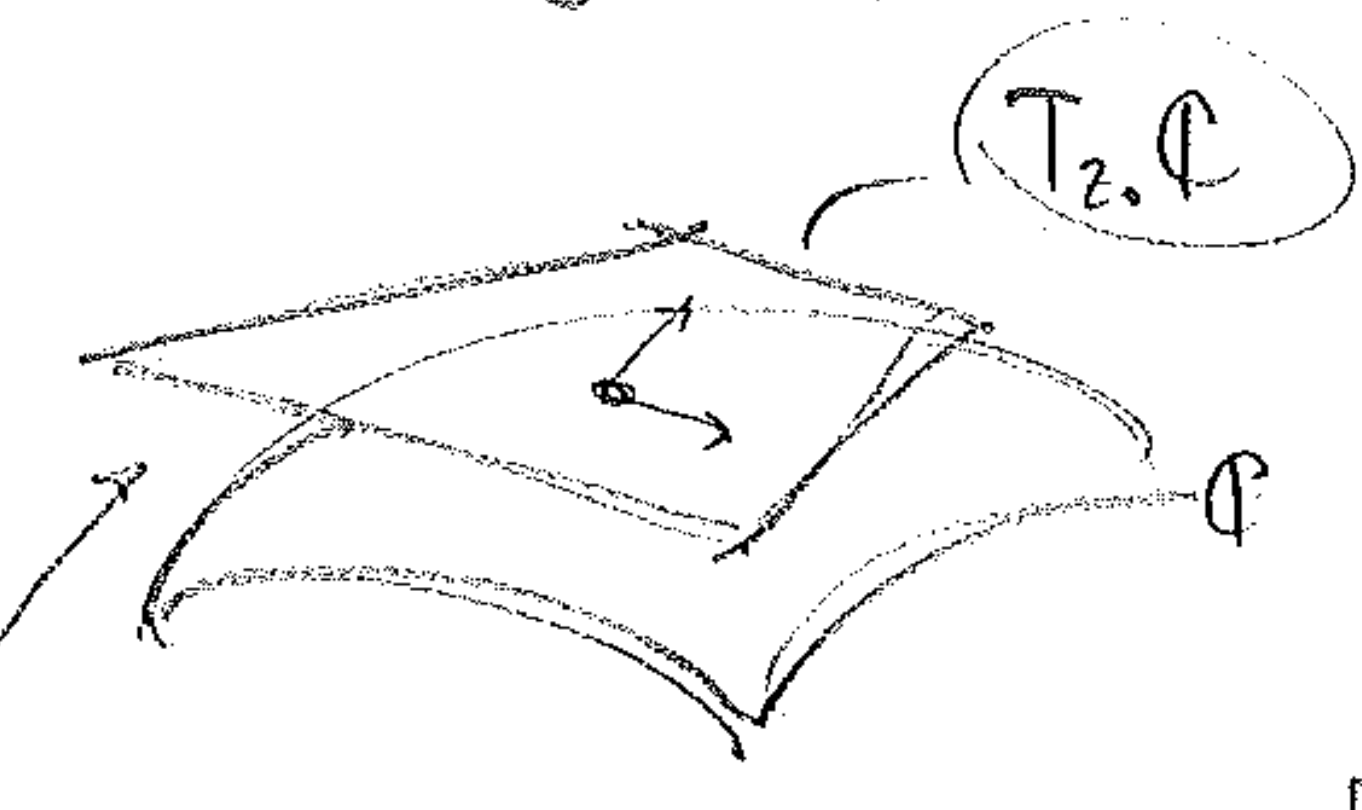
\includegraphics[width=.5\textwidth]{figures/lec13_mani.png}
\end{center}
Using the jargon of differential geometry, we call the complex plane the \emph{base manifold}. The set of all tangent spaces is called a \emph{tangent bundle}\footnote{More general types of vector spaces can be attached to each point of the base manifold. These are called fiber bundles. They are the underlying mathematical structure of mechanics and reflect why Hamilton's equations are so damn special. They are also the mathematical structure that defines gauge theories and so address the question ``what is a force?''}. Each tangent space is a vector space `attached' to a single point of the base space. 

The object $df(z_0)$ is a dual vector on the vector space\footnote{The standard notation is to write a dual vector of a space $V$ as a vector in the dual space $V^*$, so one could write $df(z_0) \in T^*_{z_0}(\mathbbm{C})$.} $T_{z_0}(\mathbbm{C})$.  The vectors of this space are `velocities' of trajectories that pass through $z_0$. For now let's think of them as quantities
\begin{align}
	\vec v = \Delta x + i \Delta y \ .
\end{align}
\begin{center}
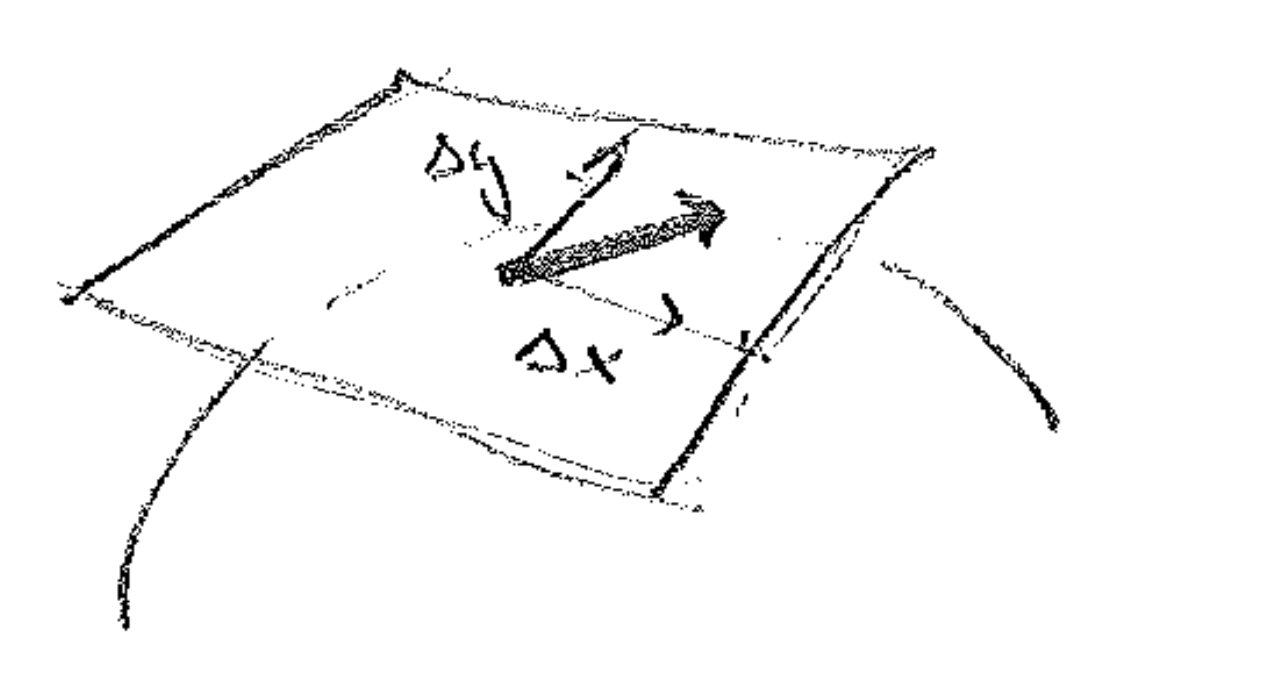
\includegraphics[width=.5\textwidth]{figures/lec13_tanvec.png}
\end{center}
Then we may write the linear action of $df(z_0)$ on $\vec v \in T_{z_0}(\mathbbm{C})$ as
\begin{align}
	df(z_0)\left[\vec{v}\right] &=
	f'(z_0)\Delta x + f'(z_0)i\Delta y \ ,
	\label{eq:diff:geo:CR:1}
\end{align}
where we assume that $f$ is analytic so that $f'(z_0)$ is unambiguously defined (independent of the direction of $\delta z$) as in \eqref{eq:df:dz:analytic:def}. 

However, if we think about this complex space as a two-dimensional real space, the following is also true:
\begin{align}
	df(z_0)\left[\vec{v}\right] &=
	\left.\frac{\partial f}{\partial x}\right|_{z_0} \Delta x
	+
	\left.\frac{\partial f}{\partial x}\right|_{z_0} \Delta x
	\label{eq:diff:geo:CR:2}
\end{align}
Comparing \eqref{eq:diff:geo:CR:1} and \eqref{eq:diff:geo:CR:1} gives 
\begin{align}
	\frac{\partial f}{\partial x} = f'(z_0) = - i\frac{\partial f}{\partial y} \ .
\end{align}
Recalling that $f= u+iv$ then gives
\begin{align}
	\frac{\partial u}{\partial x}
	+ i
	\frac{\partial v}{\partial x}
	=
	-i
	\frac{\partial u}{\partial y}
	+
	\frac{\partial v}{\partial y} \ .
\end{align}
Setting the real and imaginary parts equal to one another give, as expected, the Cauchy--Riemann equations. 

\subsection{Analytic and harmonic}

One more comment is in order. If a function $f(z) = u(x,y)+ i v(x,y)$ is analytic, then its real and imaginary parts are independently 2D harmonic with respect to $\mathbbm{R}^2$:
\begin{align}
	\partial_x^2 u(x,y) + \partial_y^2 u(x,y) &= 0
	&
	\partial_x^2 v(x,y) + \partial_y^2 v(x,y) &= 0 \ .
\end{align}
Harmonic functions show up all over the place---though admittedly you probably care mostly about three-dimensional harmonic functions. The above realization may be helpful, however, for 3D systems for which the third dimension is trivial. For example, you may want to consider fluid flow across an airplane wing. One can take the limit where the wing is infinitely long so that the fluid dynamics reduces to the two-dimensional motion around a cross section of the wing. Alternatively, maybe you care about an electrostatic system which are similarly `effectively' 2D. In this case you can `promote' your real harmonic variable (a fluid dynamics potential or electrostatic potential) to an analytic function and then bear the full power of complex analysis to attack the problem. One of the most fascinating---if outdated---methods is called \textbf{conformal mapping} by which one can solve for a harmonic function with weird boundary conditions by mapping to much simpler boundary conditions. This topic is beautiful and gives a first, intuitive example of \emph{conformal transformations} which are a pillar of theoretical physics (in any discipline). The technique is how engineers in the pre-personal computer era designed airplane wings. For experimentalists, it is pretty neat that \acro{UCR}'s own Nathan Gabor has created an analogous micromagnetic `solver' of this very same problem\footnote{\url{https://arxiv.org/abs/2002.07902}}.

\subsection{Complex functions as maps}

A complex function $f(z)$ takes in a complex number and returns a complex number. These are maps of the complex plane to itself. It is useful to build an intuition for this rather trivial-sounding statement: complex functions `deform' the complex plane. 

\begin{example}
Consider the function that multiplies a complex number by a constant phase,
\begin{align}
	f(z) = e^{i\theta} z \ .
\end{align}
This takes each point and rotates it in the counterclockwise direction by $\theta$. 
\begin{center}
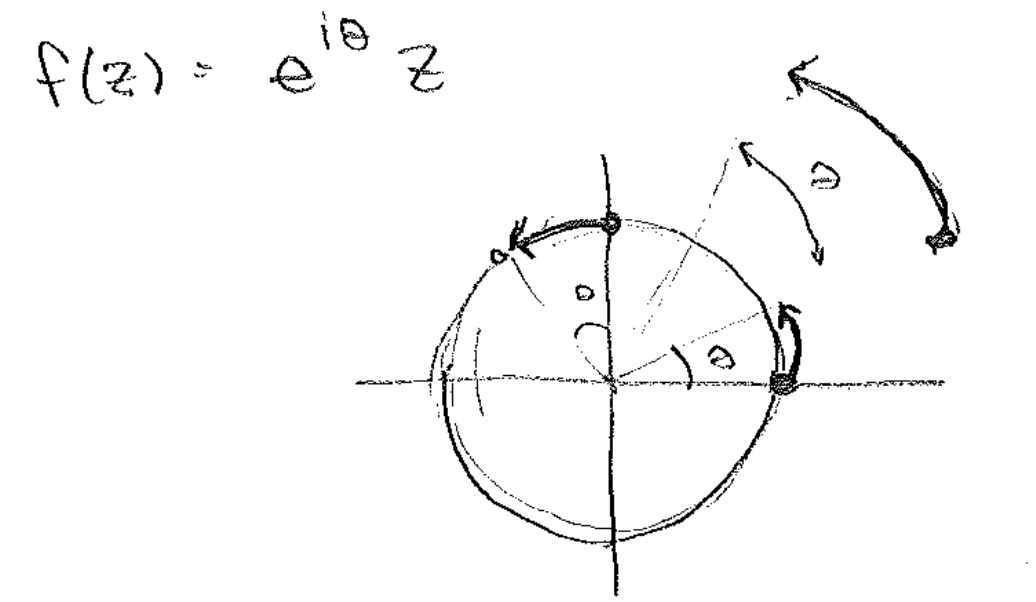
\includegraphics[width=.5\textwidth]{figures/lec13_map1.png}
\end{center}
\end{example}

\begin{exercise}
What happens to points under $f(z) = z+ z_0$?
\end{exercise}


\begin{example}
Now consider the simplest non-trivial polynomial, the function that squares its argument:
\begin{align}
	f(z) =  z^2 \ .
\end{align}
For a point $z = \rho e^{i\theta}$, $f(z)  = \rho^2 e^{2i\theta}$. This squares the modulus (length) of each point and rotates according to how much the point is already rotated relative to the positive real axis.
\begin{center}
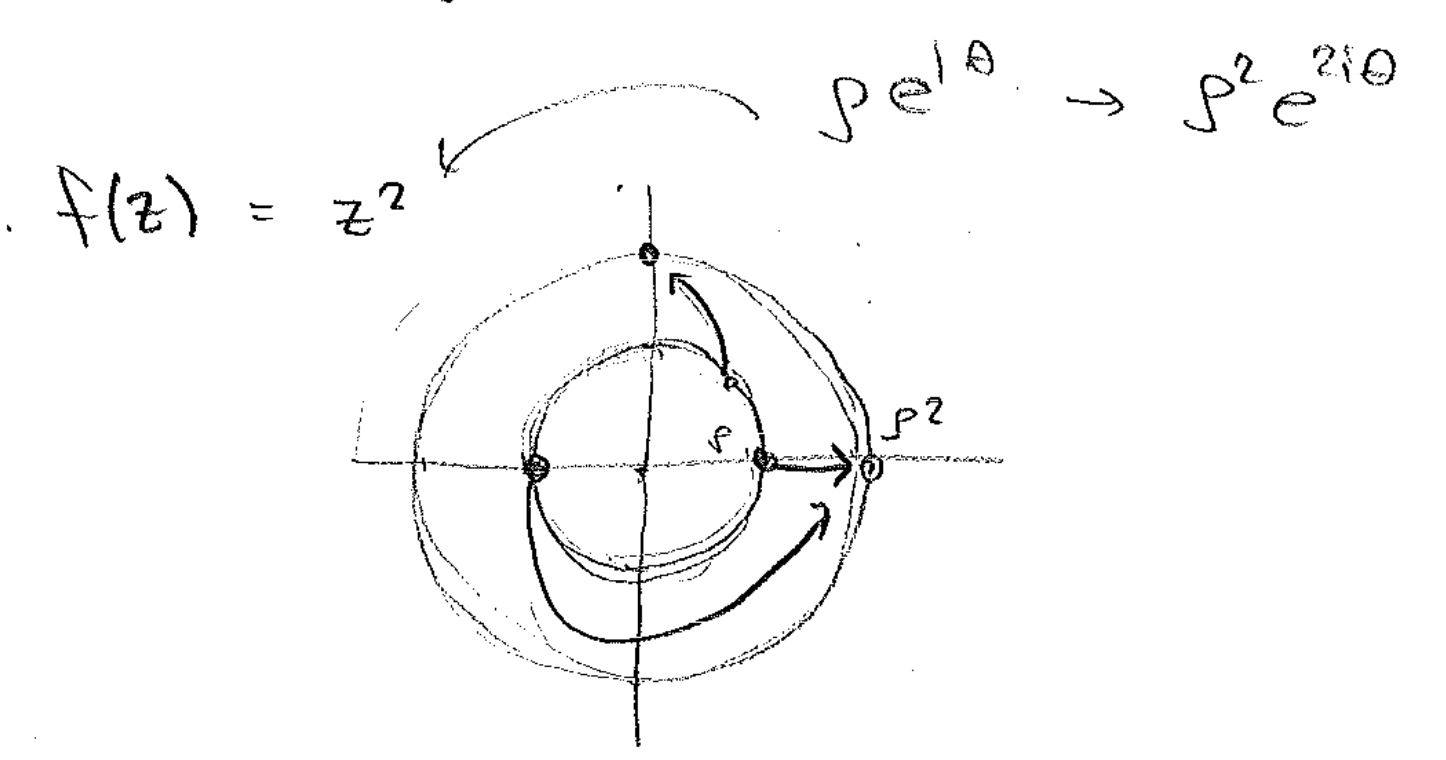
\includegraphics[width=.7\textwidth]{figures/lec13_map2.png}
\end{center}
Points that are inside the unit circle get pulled closer to the origin while points outside the unit circle are pushed away from the origin.  Points in the first quadrant (positive real and imaginary parts) are sent to points in the upper half plane (positive imaginary part).
\end{example}

\begin{exercise}
Show that under the map $f(z)=z^2$, a vertical line gets mapped onto a parabola:
\begin{center}
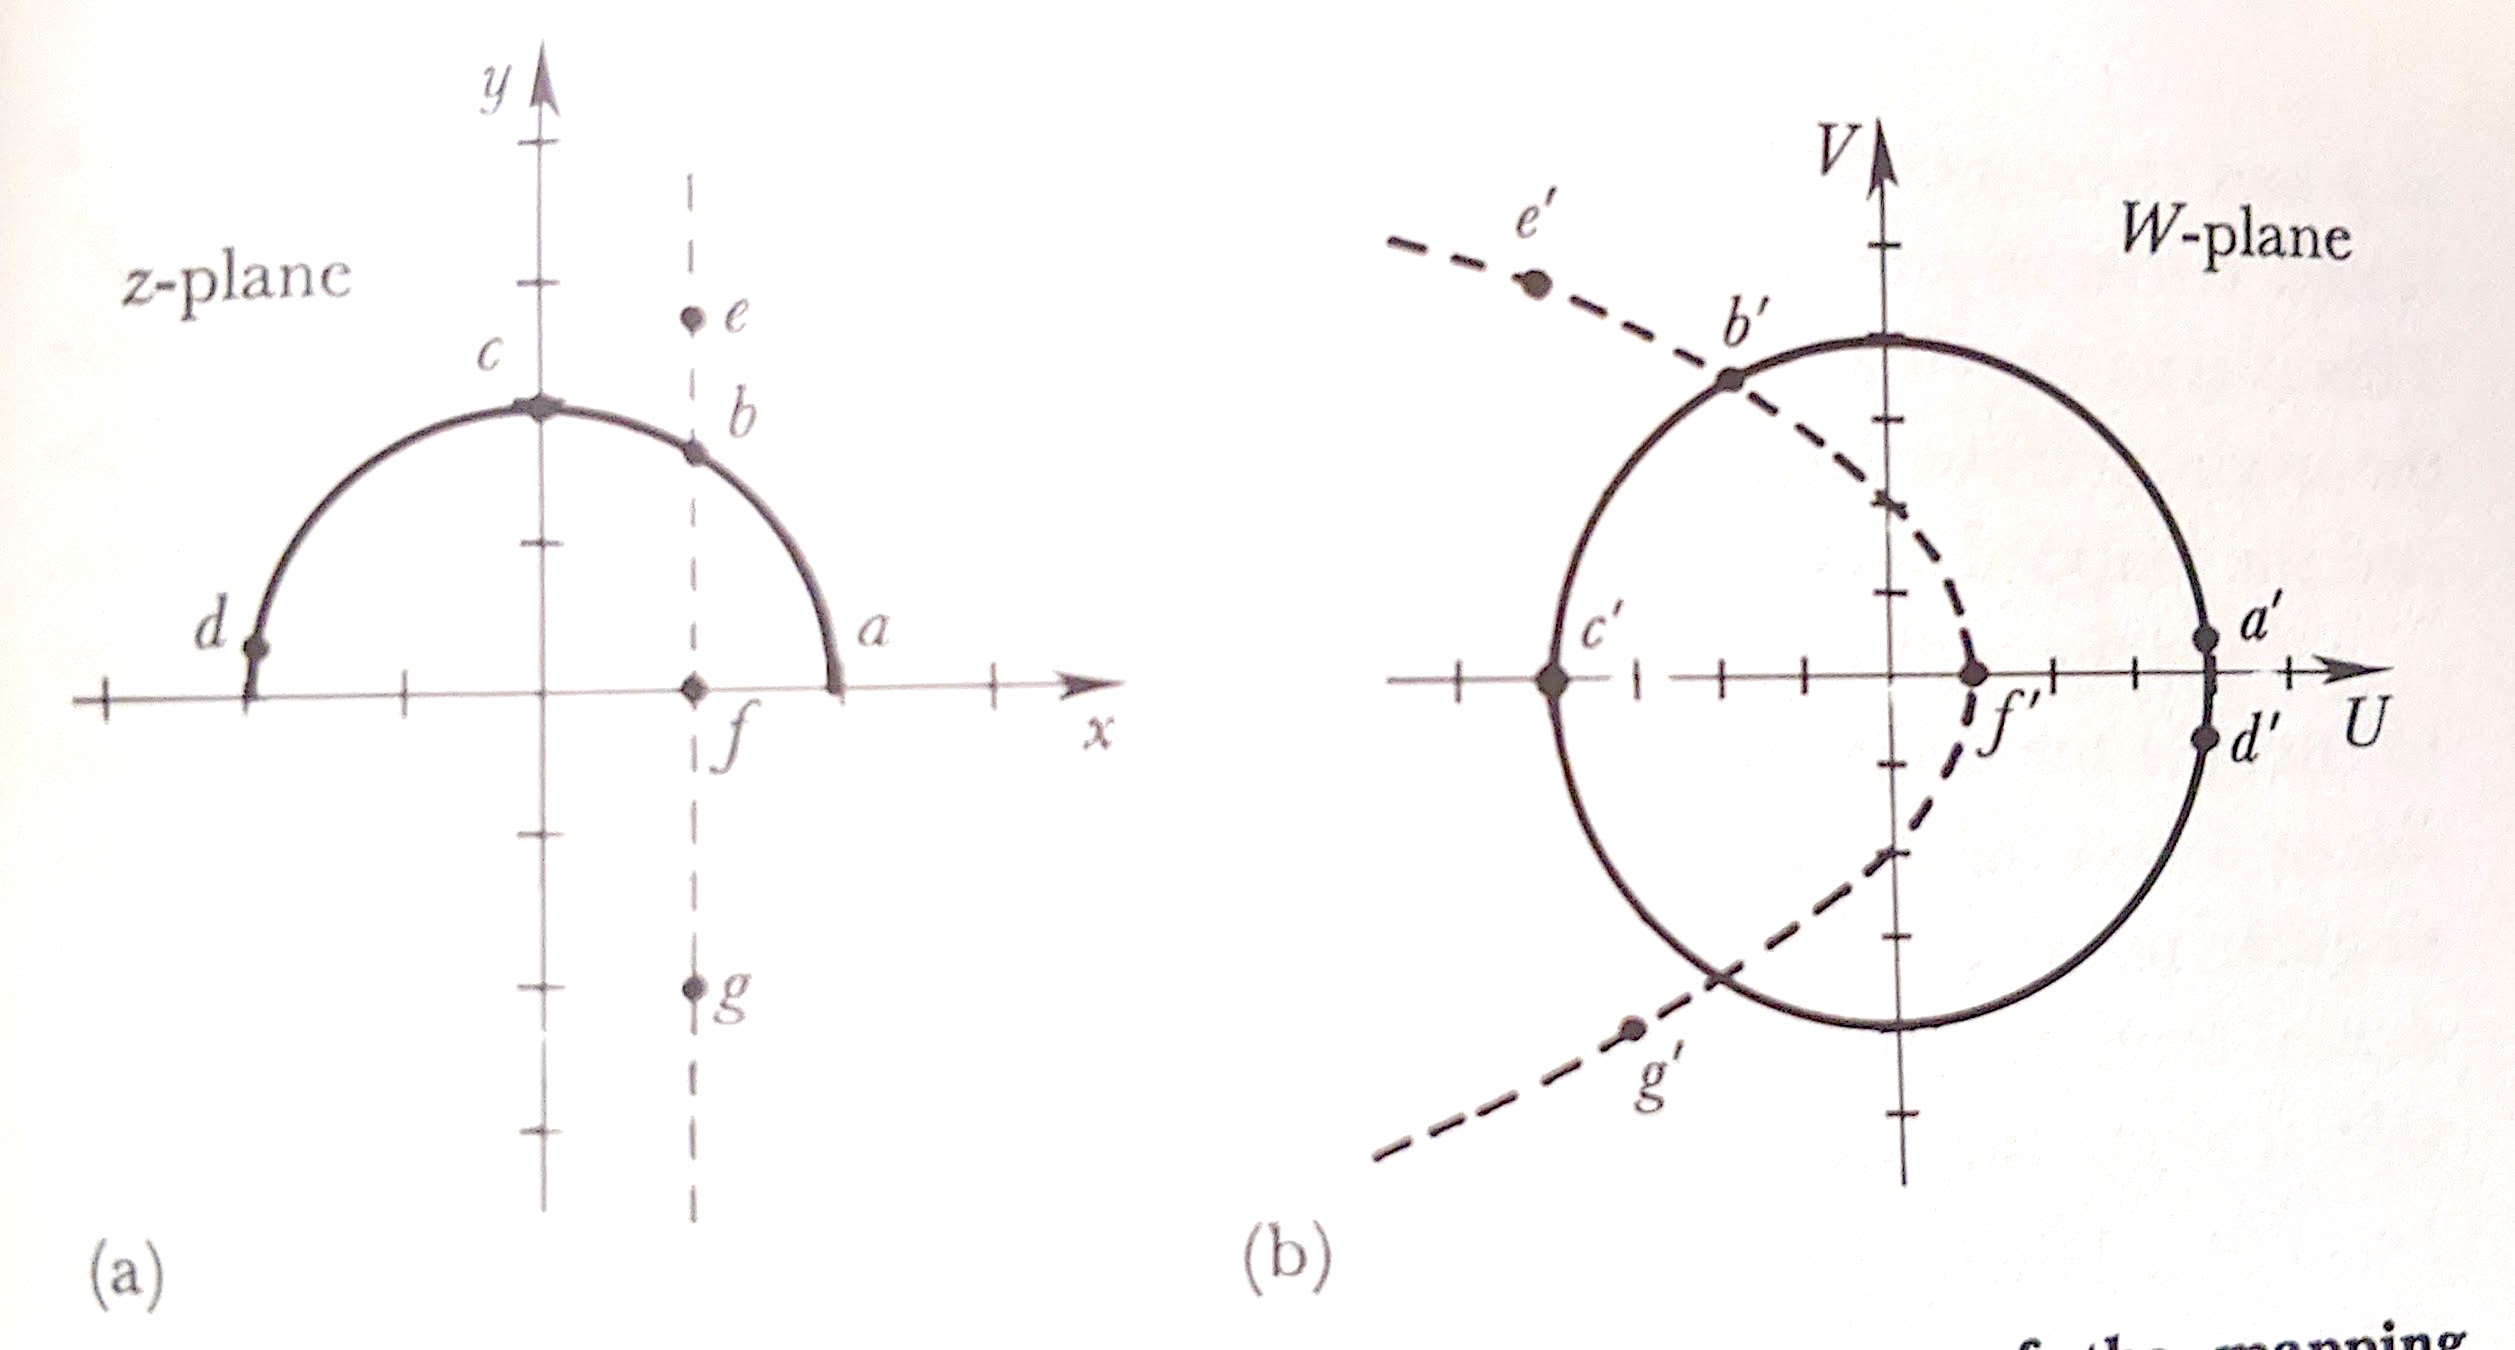
\includegraphics[width=.7\textwidth]{figures/lec13z2.jpg}
\end{center}
Figure from Matthews and Walker, points $a$, $b$, etc.\ are mapped onto $a'$, $b'$ etc. The $W$-plane corresponds to the image of the complex plan under $z^2$.
\end{exercise}

Now let's consider a curious case. What about the square root function?
\begin{align}
	f(z) = \sqrt{z} \ .
\end{align}
Something very weird happens here. Consider a closed path $\gamma(t) = e^{it}$ with path parameter $t \in [0,2\pi]$. This just means consider a bunch of points corresponding to $\gamma(t)$ with a bunch of values of $t$ in the specified range. Clearly this corresponds to a circle. However, when we put those points through the square root function, these only map onto \emph{half} of the circle. 
\begin{center}
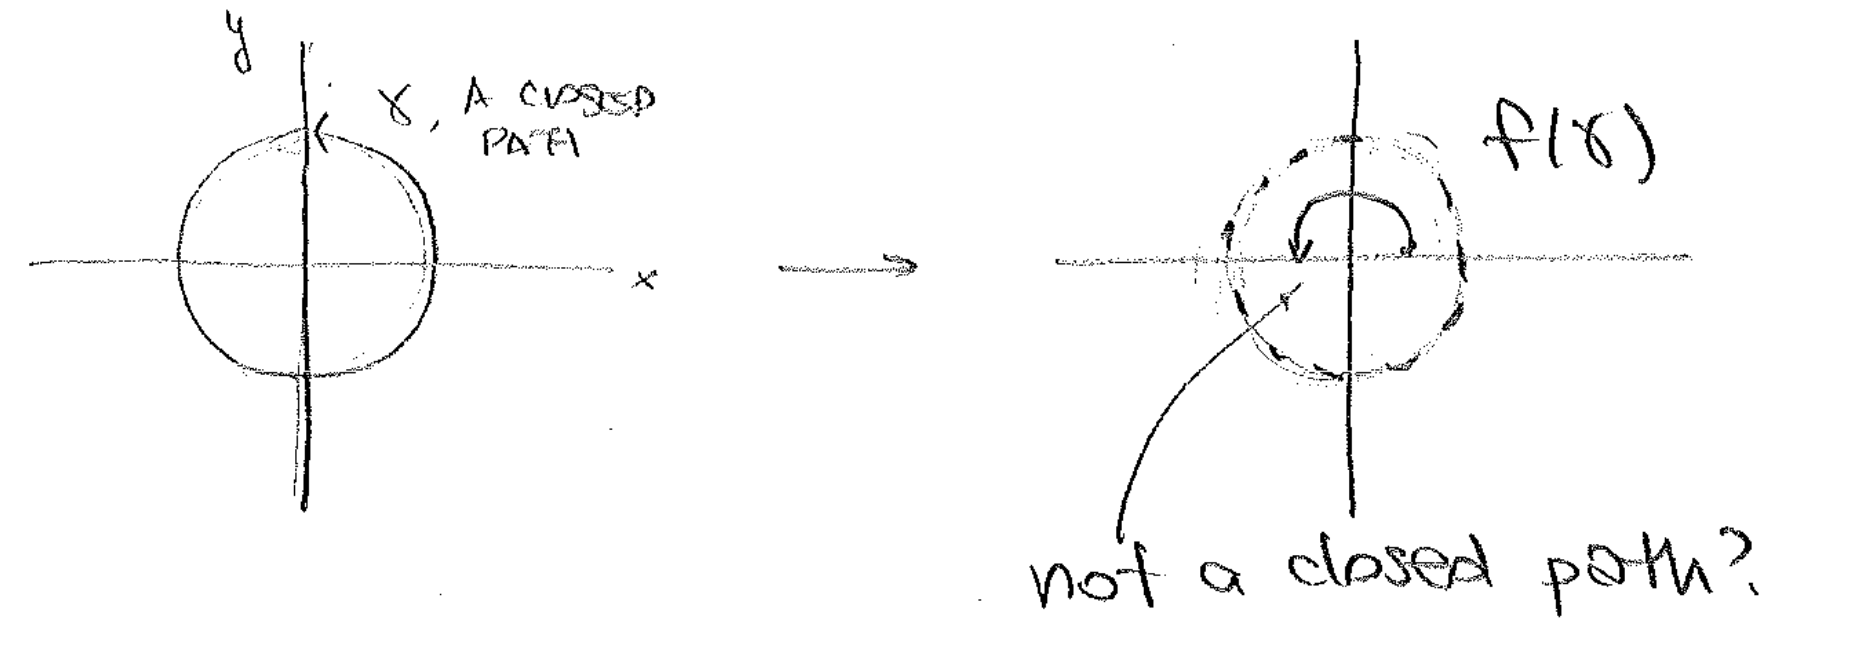
\includegraphics[width=\textwidth]{figures/lec13_map3.png}
\end{center}
The technical fact that this happens is not surprising at all, you can see that $f(\gamma(t)) = e^{it/2}$ which only spans the upper half circle. But a deeper question bubbles to the surface: if we're thinking about complex functions as maps of the complex plane to itself, what does it mean that $f(z) = \sqrt{z}$ appears to have `lost' the entire lower half of $\mathbbm{C}$? Or more strangely, how is it that a \emph{closed path} has been mapped to an \emph{open path} with endpoints?

It's clear that if we wanted to reach the \emph{lower} half plane in the iamage, we'd need $\theta \in [0, 4\pi]$. Algebraically that means that $f(\gamma(t)) = e^{it/2}$ covers the entire complex plane \emph{only} if we allow angles from 0 to $4\pi$
\footnote{You may be familiar with another case where `rotating by $2\pi$' only takes you halfway---spinors in relativistic quantum mechanics. You should know that the `double cover' nature of the spinor is (to the best of my view) independent of the present discussion of Riemann sheets. That double cover has to do with the universal cover of the Poincar\'e group. I refer to the literature on the Wigner theorem, see e.g.\ volume 1 of Weinberg's \emph{Quantum Theory of Fields}. For an unrelated cute spinor paper, see \url{https://www.jstor.org/stable/2318771}.}. In some sense, this is totally ridiculous, since $\rho e^{i\theta} \equiv \rho e^{i(\theta+2\pi)}$. I put that third bar on the equal sign because they're supposed to be \emph{that} equal.

If, say, $z_1=e^{i\pi/3}$ and $ z_2 e^{7i\pi/3}$ are supposed to be the \emph{same} point, $z_1\equiv z_2$, how is it that $f(z_1) = e^{i\pi/6}$ and $f(z_2) = e^{7i\pi/6}$ so that $f(z_1)\neq f(z_2)$? Stated differently, functions are supposed to be single valued. It appears that $f(z)=\sqrt{z}$ is \emph{multivalued} since the same point $z_1=z_2$ is mapped onto two different points. One way to do this is to \emph{define} additional structure and extend the domain (pre-image) of $f$. In order to do this, we take \emph{two} copies of the complex plane and stitch them together:
\begin{center}
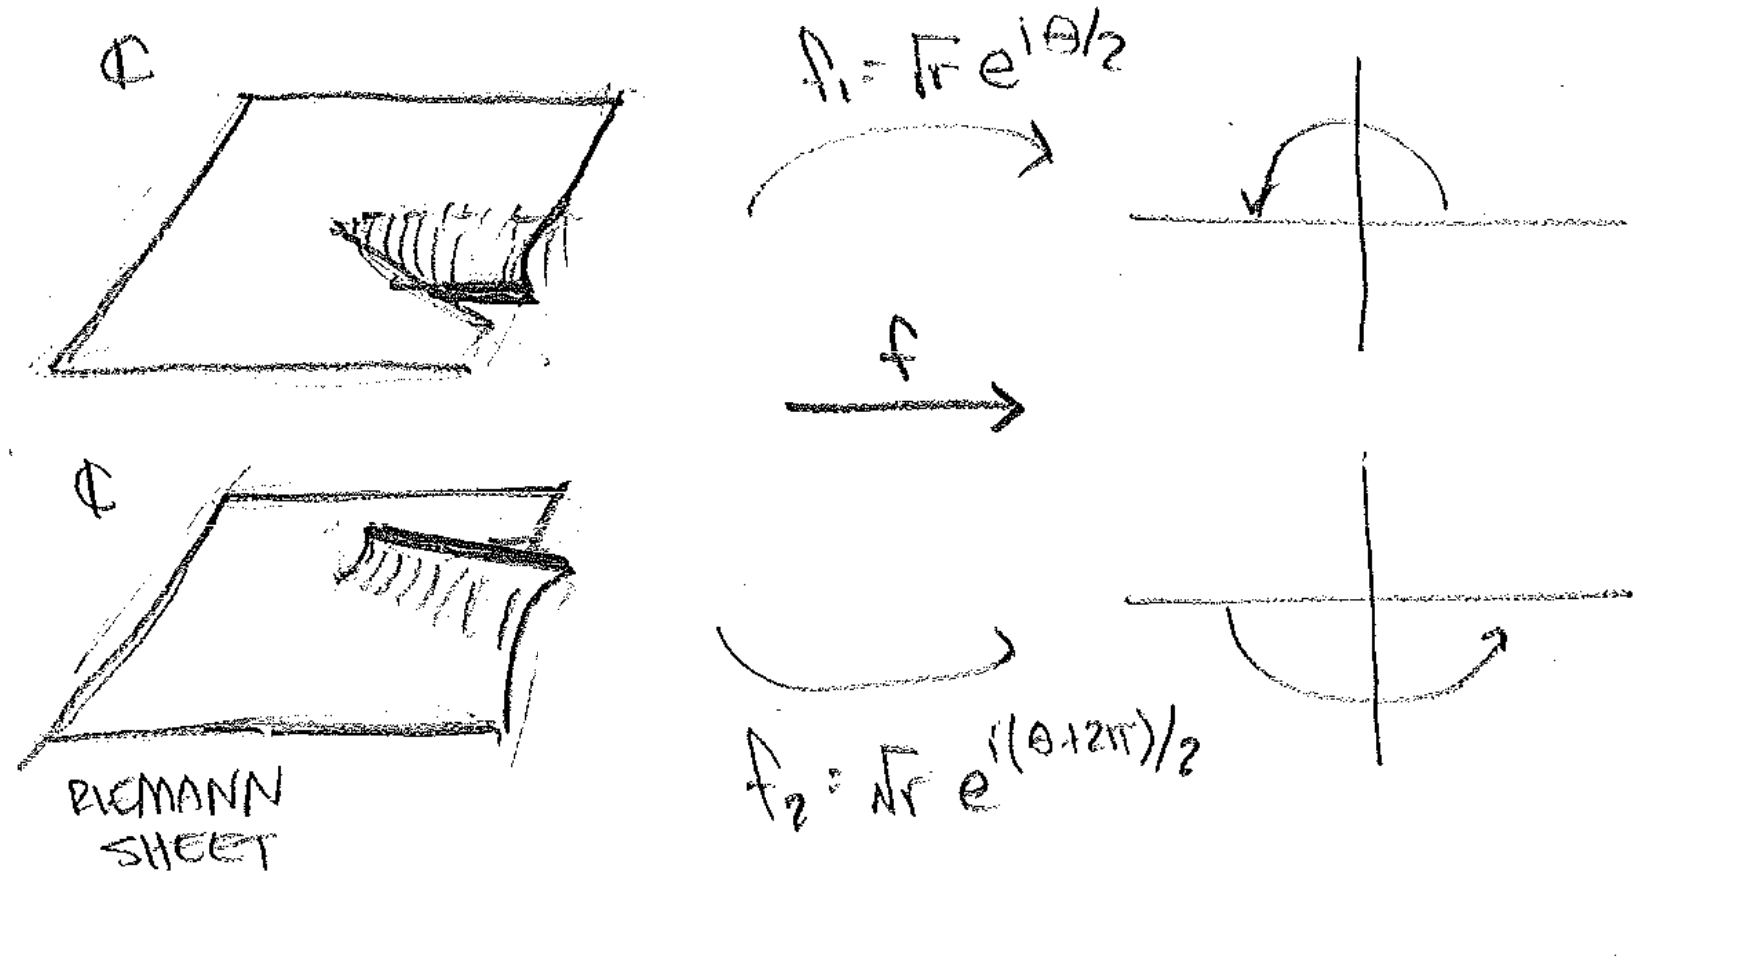
\includegraphics[width=.8\textwidth]{figures/lec13_map4.png}
\end{center}
Each copy of the complex plane is called a \textbf{Riemann sheet}. We `glue' these sheets together by defining that $\rho e^{i(\theta+2\pi)}$ of one sheet maps onto $\rho e^{i\theta}$ of the other sheet. Implicitly this chooses the positive real axis as a place where we \emph{cut} each sheet and glue them together. We call this a \textbf{branch cut}. One could, of course, have chosen the domain of each sheet to be any interval, say $\theta \in [-\pi,\pi]$ and picked a different branch cut ($\theta_\text{branch} = \pi$). 
\begin{exercise}
Is $f(z)=\sqrt{z}$ analytic on the extended complex plane (two Riemann sheets glued together at, say, $\theta=2\pi$)?
\end{exercise}
Take a moment to ponder the above exercise. As you may suspect, the relevant question isn't whether a function $f(z)$ `is analytic,' but rather \emph{where} is that function analytic? Is it analytic (differentiable) anywhere? Sure---when stay within one Riemann sheet, say $\theta\in (0,2\pi)$ and staying away from the boundary, $f(z)=\sqrt{z}$ is perfectly differentiable. Further, there's nothing special about the branch cut---we could have placed it anywhere. Thus it doesn't seem like there's \emph{any} place at which $f(z)$ is \emph{not} analytic. 

This should make sense: analyticity is about whether a function is differentiable at a given point. This is inherently a \emph{local} notion. The misbehavior of $f(z)=\sqrt{z}$---the necessity of Riemann sheets and a branch cut---are \emph{global} issues when we try to explore the \emph{whole} space. The interplay between local properties (like derivatives and Taylor expansions) and global properties (like integrals over a closed surface or topology) is a critical theme in mathematical physics. The function $f(z) = \sqrt{z}$ is analytic everywhere, but that doesn't mean we don't have to be careful. One of the lessons from this section is that the existence of a branch cut can be critically important if you happen to take trajectories that are \emph{loops} in the complex plane. For those who know where this is going: whenever there are branch cuts, you have to be careful with your contour integrals. This typically happens whenever you have a function that is not some series of integer powers of $z$.

As a final example, let's consider the complex logarithm. We'll use the notation of Byron and Fuller and write $\log$ to denote the complex natural logarithm and $\ln$ to denote the `usual' natural logarithm acting on real numbers. For $z=r e^{i\theta}$, the complex logarithm satisfies
\begin{align}
	\log z &= \ln r + i \theta
	\\
	\log(z_1z_2)
	&=\ln(r_1r_2) + i (\theta_1+\theta_2)
	= \log z_1 + \log z_2 \ .
\end{align}
\begin{example}
What does the domain of the complex logarithm look like? As a function, $f(z) = u(z) + i v(z)$, we see that $v(z) = \theta$ and $v(z_1z_2)=\theta_1+\theta_2$. This means that if we take a trajectory that keeps going around the origin, $v(z)$ just keeps increasing\footnote{This is where you can start humming `stairway to heaven.'}. Each time you go around you must be on a new Riemann sheet. 
\end{example}
Rather than having an infinite number of Riemann sheets, an alternative way of thinking about this is to imagine an infinite number of equally valid `complex logarithm' functions labeled by $n$:
\begin{align}
	f_n(z) &= \ln r + i \theta + 2\pi n i \ .
\end{align}
\begin{center}
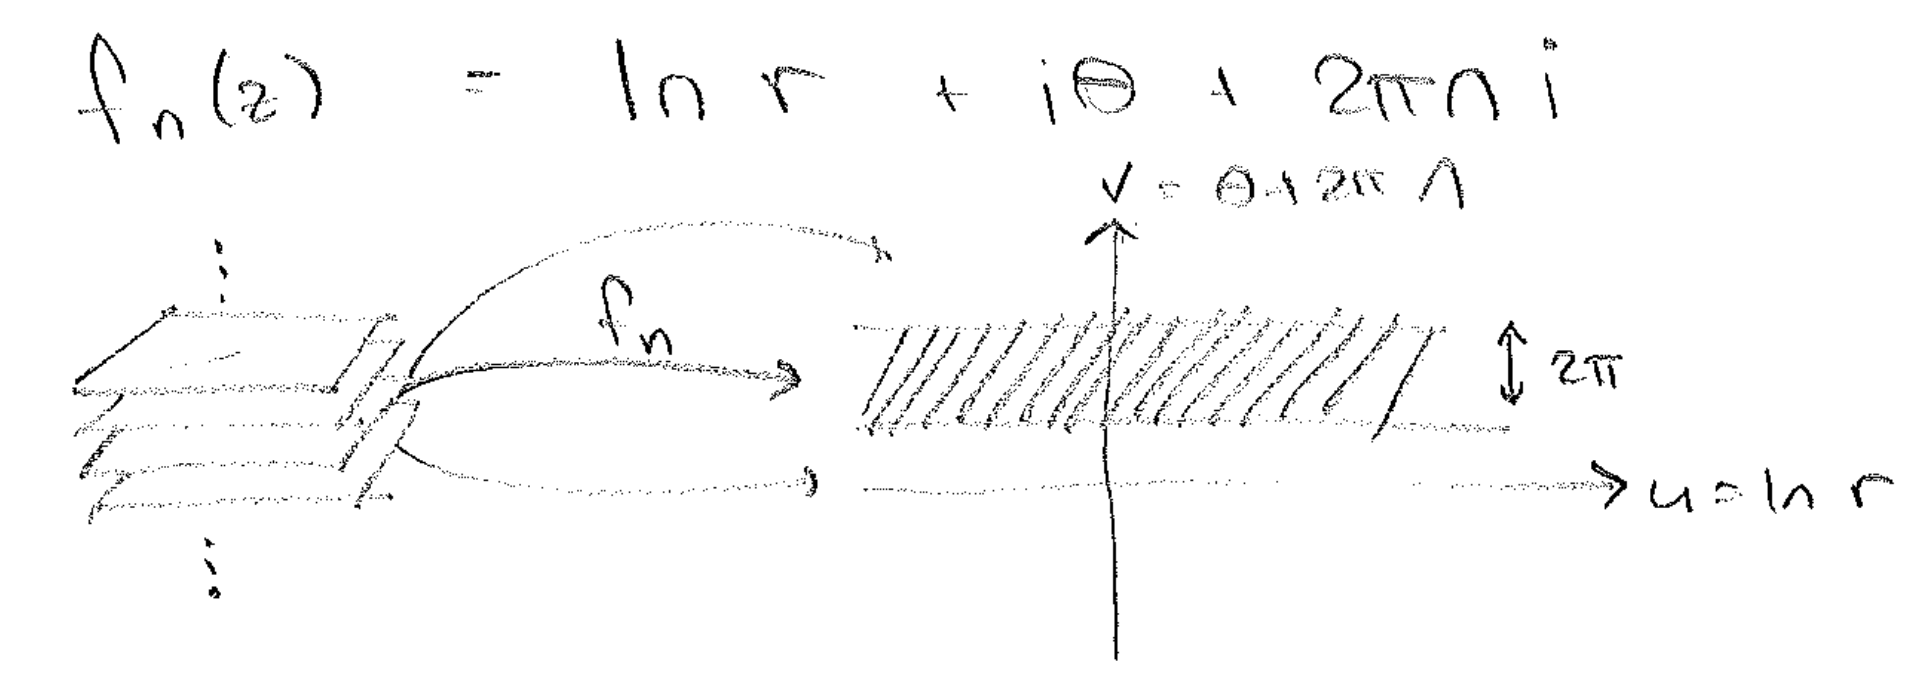
\includegraphics[width=\textwidth]{figures/lec13_map5.png}
\end{center}
The image of the $f_n(z)$ corresponds to a horizontal strip with $v\in \left(2\pi n, 2\pi(n_1)\right)$.
\begin{example}
Is the complex logarithm analytic? Everywhere but at $z=0$.
\end{example}
Let us end by repeating the main point of introducing branch cuts:
\begin{framed}
\begin{center}
Do not integrate across a branch cut!
\end{center}
\end{framed}

\subsection{Integration on the Complex Plane}
% StoGo 17.2.1

\subsection{Cauchy Integral Theorem}


